% ----------------------------------------------------------------------------------------------------- %
% Manual da Classe UFTeX
% 
% Versão 2.1:   Março 2018
%
% Criado por:   Tiago da Silva Almeida
% Revisado por: Tiago da Silva Almeida
%               Eleanor
%               Ary Henrique Morais de Oliveira
%
% https://almeidatiago.github.io/uftex/
% ----------------------------------------------------------------------------------------------------- %

\documentclass[tcc2]{uftex}
% ---- Esse comando cria o nome uftex estilizado
\newcommand\uftex{UF\TeX}

\usepackage[utf8]{inputenc} % Para suporte a caracteres especiais
\usepackage[T1]{fontenc}    % Para melhorar a formatação dos caracteres especiais
\usepackage[brazil]{babel}  % Para ajuste da língua portuguesa
\usepackage{graphicx}  % Pacote necessário para incluir imagens
\usepackage{lipsum}
\usepackage{tikz}
\usepackage[siunitx]{circuitikz}
\usetikzlibrary{arrows}
\usepackage{enumitem}

\usepackage[alf,abnt-emphasize=bf]{abntex2cite}
\renewcommand{\backrefpagesname}{}
\renewcommand{\backref}{}
\renewcommand*{\backrefalt}[4]{}

% ----  Esses comandos são necessários no pré-ambulo para a impressão da lista de abreviaturas e de símbolos
\makelosymbols
\makeloabbreviations
% ---- Início do documento
\begin{document}

  % ---- Descrição do título do trabalho 
  \title{Análise Empírica de Algoritmos de Ordenação}
  % ---- Nome do autor ou autores do trabalho
  \author{Daniel}{Vinicius da Silva, Érick Santos Marçal, Benedito Jaime Melo Moraes Junior}
  % ---- Nome do orientador do trabalho. O último campo representa o título do professor
  \advisor{Prof.}{Tiago}{da Silva Almeida}{Me.}

  \examiner{Prof.}{Dr.}{Nome do Primeiro Examinador Sobrenome}
  \examiner{Profa.}{Dra.}{Nome do Segundo Examinador Sobrenome}
  \examiner{Profa.}{Ma.}{Nome do Terceiro Examinador Sobrenome}
  % ---- Departamento representa o curso ao qual o trabalho está sendo apresentado. Descrito por meio de duas iniciais do curso
  \department{CC}
  % ---- Data da apresentação do trabalho
  \date{06}{06}{2024}
  % ---- Palavras-chaves em português do trabalho
  \keyword{\LaTeX}
  \keyword{\uftex}
  \keyword{Trabalho de Conclusão de Curso}
  \keyword{Redação Científica}
  \keyword{Extensão Universitária}
  % ---- Palavras-chaves em inglês do trabalho
  \foreignkeyword{\LaTeX}
  \foreignkeyword{\uftex}
  \foreignkeyword{Bachelor Thesis}
  \foreignkeyword{Scientific Writing}
  \foreignkeyword{University Extension}
  
  % ---- Comando responsável por criar a capa do trabalho, logo em seguida está o comando que insere a folha de rosto conforme a configuração exigida
 \maketitle

% Esse comando Insere a Folha de Rosto
  % \frontmatter

  % ----------------------------------------------------------------------------------------------------- %
  %  Este trecho deve ser inserido somente no caso do TCC2 já na versão FINAL
  % ----------------------------------------------------------------------------------------------------- %
  % \includepdf{ficha_catalografica}
  
  % ----------------------------------------------------------------------------------------------------- %
  % Esse comando insere a Folha de Aprovação
  % \makepageapprove
  
  % A Ata de aprovacao nao deve fazer parte do TCC 2, mas deve-se incluir a folha de aprovacao assinada pelos membros da banca
  %\includepdf{ata_de_aprovacao}
  % ----------------------------------------------------------------------------------------------------- %
  % \dedication{A algu\'em cujo valor \'e digno desta dedicat\'oria.}

  % \begin{acknowledgement}
  % Gostaria de agradecer a todos.
  % \end{acknowledgement}

  % \begin{abstract}
  % \lipsum[1]
  % \end{abstract}

  % \begin{foreignabstract}
  % \lipsum[9]
  % \end{foreignabstract}
  \printlosymbols  
  \printloabbreviations
  % ---- Cria a lista de figuras. OPCIONAL
  % \listoffigures
  % ---- Cria a lista de tabelas. OPCIONAL
  % \listoftables 
  % ---- Cria o sumário. OBRIGATÓRIO
  % \tableofcontents % sumário
% --- Marca o inicio dos elementos textuais. Capítulos.
\mainmatter
% ---- Defino o espaçamento de um e meio centímetros
\onehalfspacing
% ----------------------------------------------------------------------------------------------------- %
% Capítulos do trabalho
% ----------------------------------------------------------------------------------------------------- %
\ChapterStart{first}{First chapter}
\chapter{Introdução}

A ordenação de dados é uma operação fundamental na ciência da computação e em diversas áreas aplicadas. Muitos problemas computacionais, sejam eles simples ou complexos, exigem a ordenação como uma etapa intermediária ou final. Sua importância pode ser destacada pela eficiência em busca e recuperação de dados, pelo preprocessamento necessário para outros algoritmos, pela facilidade de visualização e análise, e pela melhoria de desempenho em sistemas de gerenciamento de banco de dados e outras aplicações de grande escala.

O objetivo deste trabalho é comparar o desempenho de seis algoritmos de ordenação diferentes em termos de tempo de execução, uso de memória e facilidade de implementação. Ao fazer isso, buscamos identificar quais algoritmos são mais adequados para diferentes situações e tipos de dados. 

Especificamente, este trabalho analisará os seguintes algoritmos de ordenação:
\begin{itemize}
    \item \textbf{Bubble Sort}: Um algoritmo simples e intuitivo com complexidade temporal de $O(n^2)$. É frequentemente utilizado para fins didáticos devido à sua simplicidade.
    \item \textbf{Selection Sort}: Outro algoritmo de complexidade $O(n^2)$, conhecido pela sua simplicidade, mas não muito eficiente para listas grandes.
    \item \textbf{Insertion Sort}: Também com complexidade $O(n^2)$, é eficiente para listas pequenas ou quase ordenadas e fácil de implementar.
    \item \textbf{Merge Sort}: Um algoritmo de ordenação eficiente com complexidade $O(n \log n)$ que utiliza uma abordagem de divisão e conquista, mas requer espaço adicional.
    \item \textbf{Quick Sort}: Amplamente utilizado devido à sua eficiência média de $O(n \log n)$, embora seu desempenho dependa da escolha do pivô.
    \item \textbf{Heap Sort}: Um algoritmo eficiente com complexidade $O(n \log n)$ que utiliza uma estrutura de dados heap, trabalhando em espaço in-place.
\end{itemize}

Nos capítulos subsequentes, serão detalhados os resultados experimentais, análises e discussões sobre o desempenho desses algoritmos, assim como sugestões para trabalhos futuros.

\chapter{Revisão Teórica}

\section{Bubble Sort}
Bubble Sort é um algoritmo de ordenação in place e estável. Foi descrito por Edward Iverson em 1960. Ele compara repetidamente pares adjacentes de elementos e troca-os se estiverem na ordem errada. Este processo é repetido até que a lista esteja ordenada. Apesar de ser fácil de entender e implementar, o Bubble Sort é ineficiente para listas grandes, com uma complexidade de tempo $O(n^2)$.

\section{Selection Sort}
Selection Sort é um algoritmo de ordenação in place e instável. Foi descrito por Donald Knuth em seu livro "The Art of Computer Programming", publicado em 1968. Funciona selecionando repetidamente o menor (ou maior, dependendo da ordem desejada) elemento da lista não ordenada e trocando-o com o primeiro elemento não ordenado. Esse processo é repetido para os elementos restantes. Embora seja simples de implementar, o Selection Sort não é eficiente para listas grandes, pois tem uma complexidade de tempo $O(n^2)$.

\section{Insertion Sort}
Insertion Sort é um algoritmo de ordenação in place e estável. As primeiras descrições formais do Insertion Sort datam dos trabalhos de Donald Knuth em 1968. Ele constrói a lista ordenada um elemento por vez, comparando cada novo elemento com os elementos já ordenados e inserindo-o na posição correta. O Insertion Sort é eficiente para listas pequenas ou quase ordenadas, com uma complexidade de tempo média de $O(n^2)$. Ele é frequentemente utilizado em algoritmos híbridos e em aplicações onde a entrada é geralmente pequena ou quase ordenada.

\section{Merge Sort}
Merge Sort é um algoritmo de ordenação estável e baseado na técnica de dividir e conquistar. Foi desenvolvido por John von Neumann em 1945. O algoritmo divide repetidamente a lista ao meio até que cada sublista contenha apenas um elemento. Depois, ele combina essas sublistas de forma ordenada para produzir sublistas maiores, até que a lista inteira esteja ordenada. O Merge Sort é eficiente e tem uma complexidade de tempo O(n log n), sendo bastante usado em situações onde a estabilidade da ordenação é crucial.

\section{Quick Sort}
Quicksort é um algoritmo de ordenação in place e instável, descrito pela primeira vez nos trabalhos do programador britânico C. A. R. Hoare em 1962. Baseia-se no princípio de dividir um problema em dois subproblemas mais simples, que são resolvidos recursivamente até que se tornem problemas triviais.

\section{Heap Sort}
Heap Sort é um algoritmo de ordenação in place e instável. Foi desenvolvido por J. W. J. Williams em 1964. Baseia-se na estrutura de dados heap, especificamente em um heap máximo ou mínimo, para ordenar os elementos. O algoritmo primeiro constrói um heap a partir da lista de elementos e, em seguida, remove repetidamente o maior (ou menor) elemento do heap, reconstruindo o heap até que todos os elementos estejam ordenados. O Heap Sort tem uma complexidade de tempo O(n log n) e é eficiente tanto em termos de tempo quanto de espaço.

\chapter{Metodologia}

Para a realização de comparação dos algoritmos foi determinado uma linguagem padrão para a implementação de todos eles, de forma que todos os algoritmos fossem executados em ambientes similares para evitar imprecisões nos dados coletados. 

\section{Descrição do Hardware}

Os testes foram realizados em dois computadores de especificações diferentes, variando na quantidade de memória RAM e até marcas de processadores.

\subsection{Notebook Dell Inspiron 15 3520}
\begin{itemize}[label=--]
    \item Processador: Intel(R) Core(TM) i5-1235U
    \item Memória RAM: 16GB DDR4 (2x8GB)
\end{itemize}

\subsection{Notebook Lenovo Ideapad Gaming 3i}
\begin{itemize}[label=--]
    \item Processador: 11th Gen Intel(R) Core(TM) i5-11300H 3.11 GHz
    \item Memória RAM: 24GB DDR4 (1x8GB, 1x16GB)
\end{itemize}

\section{Descrição do Software}

Em relação ao software utilizado, os sistemas operacionais e a versão da linguagem utilizada foram variadas.

\subsection{Notebook Dell Inspiron 15 3520}
\begin{itemize}[label=--]
    \item Sistema Operacional: Windows 11 Home 23h2
    \item Versão do Python: 3.12.3
\end{itemize}

\subsection{Notebook Lenovo Ideapad Gaming 3i}
\begin{itemize}[label=--]
    \item Sistema Operacional: Gentoo Linux 23.0 (WSL2) no Windows 11 Pro 23h2
    \item Versão do Python: 3.12.3
\end{itemize}


\section{Implementação dos Algoritmos}

Os algoritmos foram implementados utilizando a linguagem de programação Python. A escolha do Python se deve à sua simplicidade e ao seu amplo uso em ambientes acadêmicos e de pesquisa. 
Cada algoritmo foi encapsulado em uma função que recebe como entrada uma lista de números e retorna uma tupla contendo a lista ordenada, o número de comparações realizadas e o número de trocas efetuadas. Essa abordagem permite uma avaliação detalhada do desempenho de cada algoritmo, tanto em termos de tempo de execução quanto em operações realizadas.

% Insere uma imagem
\begin{figure}[h!]
    \centering
    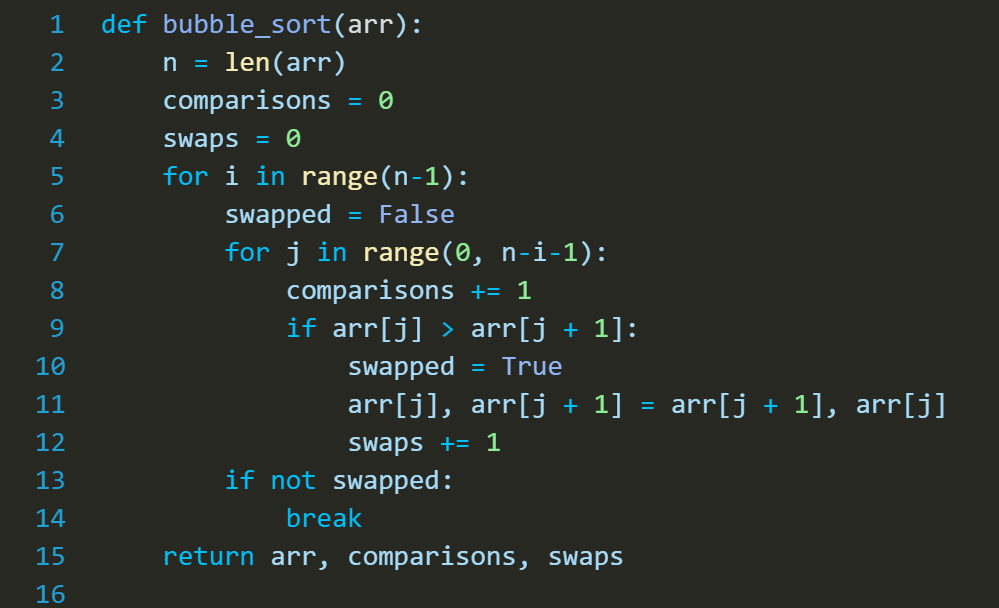
\includegraphics[width=0.7\textwidth]{bubble_sort.png}  % Substitua pelo caminho da sua imagem
    \caption{Algoritmo Bubble Sort}
    \label{fig:exemplo}
\end{figure}

\begin{figure}[h!]
    \centering
    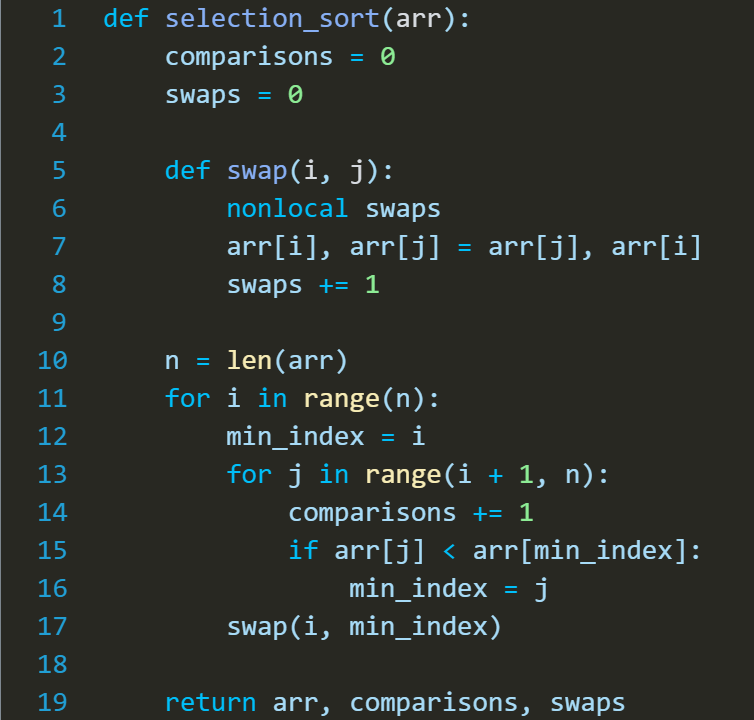
\includegraphics[width=0.5\textwidth]{selection_sort.png}  % Substitua pelo caminho da sua imagem
    \caption{Algoritmo Selection Sort}
    \label{fig:selection_sort}
\end{figure}


% Insere uma imagem
\begin{figure}[h!]
    \centering
    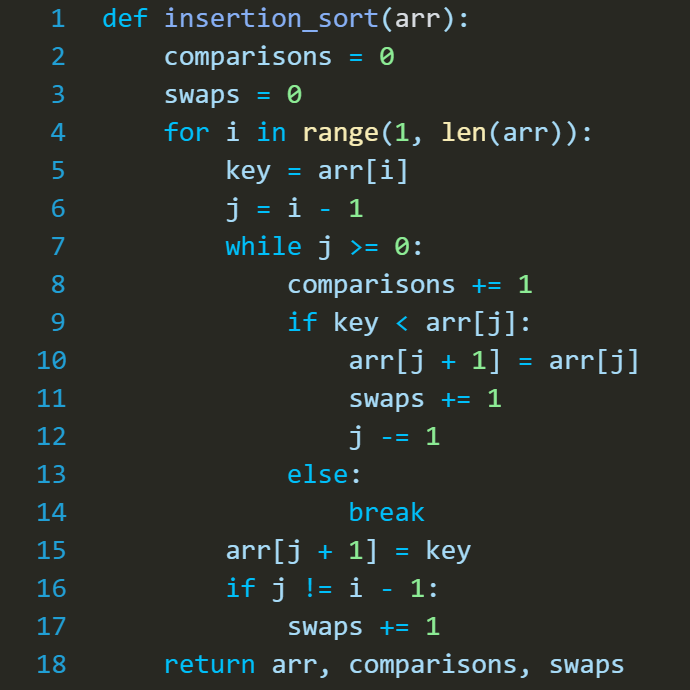
\includegraphics[width=0.5\textwidth]{insertion_sort.png}  % Substitua pelo caminho da sua imagem
    \caption{Algoritmo Insertion Sort}
    \label{fig:exemplo}
\end{figure}

% Insere uma imagem
\begin{figure}[h!]
    \centering
    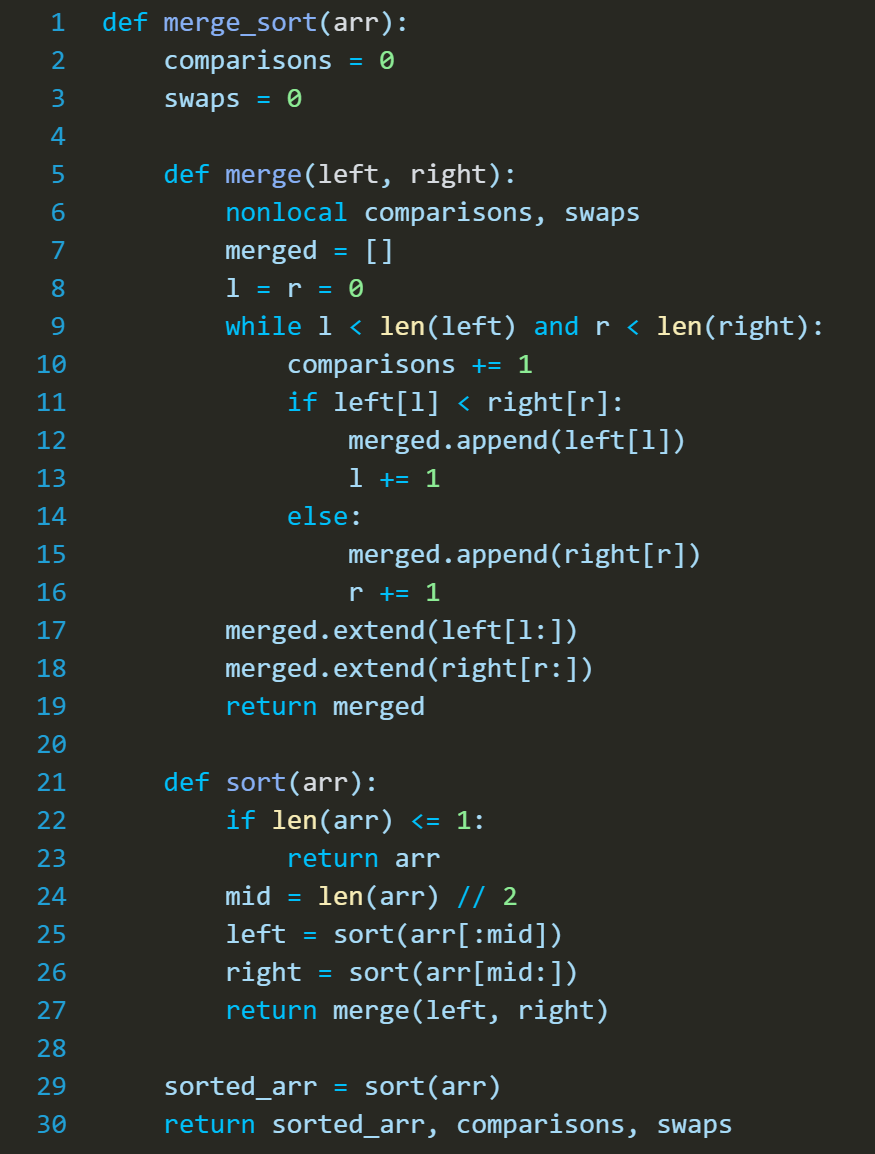
\includegraphics[width=0.5\textwidth]{merge_sort.png}  % Substitua pelo caminho da sua imagem
    \caption{Algoritmo Merge Sort}
    \label{fig:exemplo}
\end{figure}

% Insere uma imagem
\begin{figure}[h!]
    \centering
    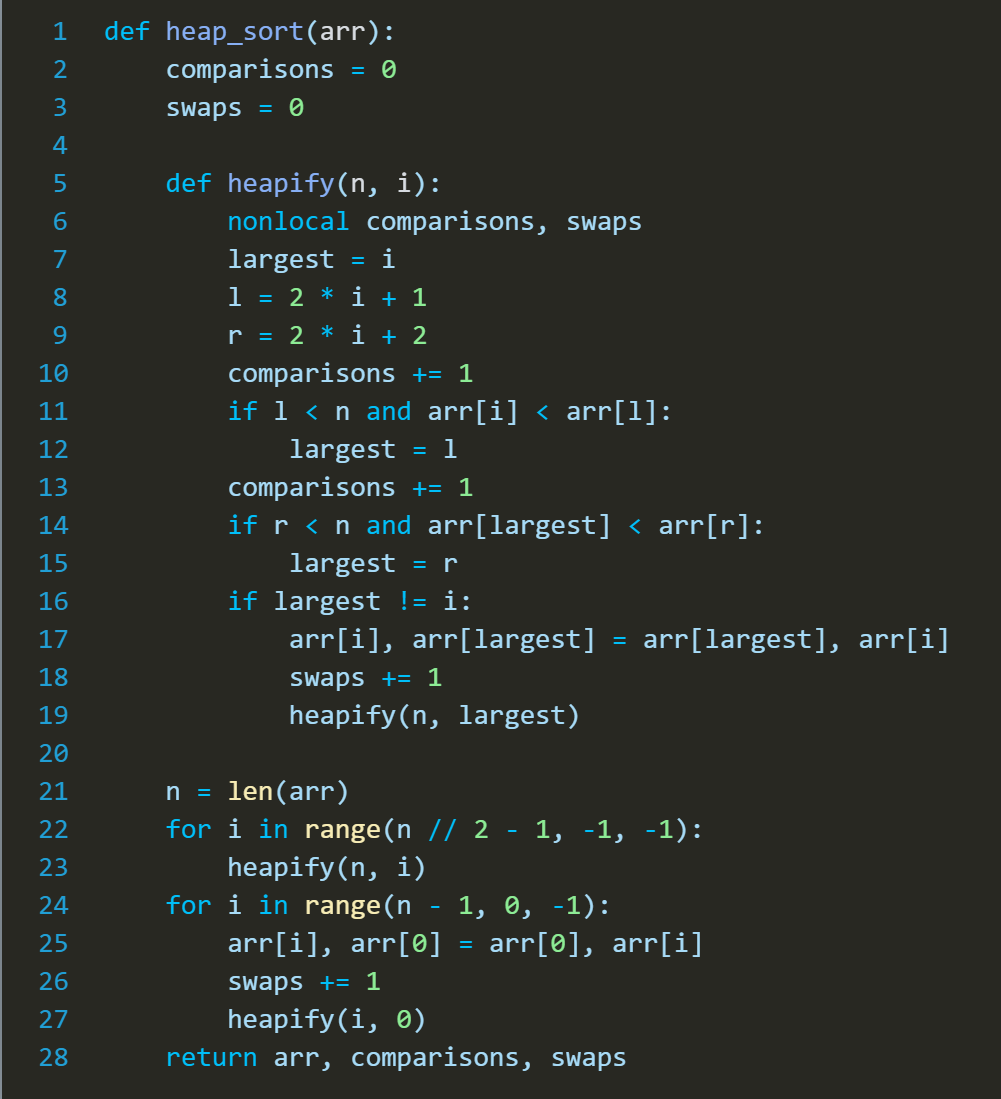
\includegraphics[width=0.5\textwidth]{heap_sort.png}  % Substitua pelo caminho da sua imagem
    \caption{Algoritmo Quick Sort}
    \label{fig:exemplo}
\end{figure}


% Insere uma imagem
\begin{figure}[h!]
    \centering
    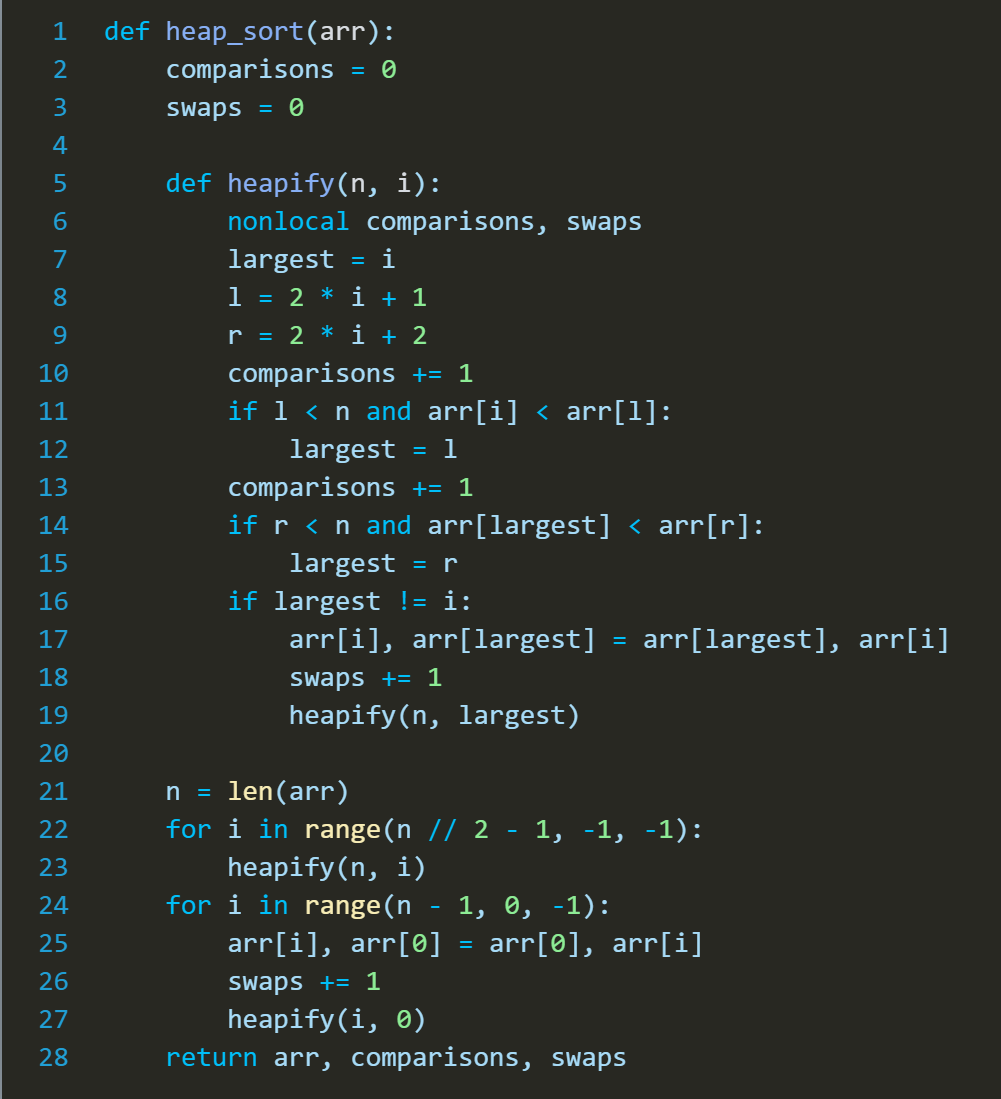
\includegraphics[width=0.5\textwidth]{heap_sort.png}  % Substitua pelo caminho da sua imagem
    \caption{Algoritmo Heap Sort}
    \label{fig:exemplo}
\end{figure}


\section{Medição do Tempo de Execução}

Para medir o tempo de execução dos algoritmos foi utilizado a função time da biblioteca padrão do Python para medir o tempo de execução dos algoritmos em milissegundos. Esse método é portátil e funciona em qualquer sistema operacional. A função é chamada antes do algoritmo de ordenação ser iniciado e após o algoritmo ser finalizado.


\section{Número de Comparações e Trocas}
Em cada função que encapsula os algoritmos, foram adicionadas duas variáveis do tipo inteiro para a realização da contagem do número de comparações e trocas, que foram incrementadas nos pontos apropriados do código.


\section{Automatização dos testes}
Para a automatização dos testes, foi criado um programa que itera a cada algoritmo uma série testes com parâmetros diferentes. Foram utilizados três tipos de listas: ordenada, inversa e aleatório. No qual cada tipo foi executado em listas com mil, dez mil, cinquenta mil e cem mil elementos.
Como cada algoritmo retorna o número de comparações e trocas, e o programa retorna o tempo em milissegundos, esses dados foram adicionados em um arquivo para análise posterior.


\chapter{Resultados}

Os resultados dos testes de desempenho dos algoritmos de ordenação são apresentados a seguir. Foram medidos o tempo de execução, o número de comparações e o número de trocas para cada algoritmo, utilizando listas de diferentes tamanhos e tipos.

% Exemplo de Tabela de Resultados
\begin{table}[h]
\centering
\label{tab:resultados}
\begin{tabular}{|l|c|c|c|c|}
\hline
\textbf{Algoritmo} & \textbf{Tipo de Lista} & \textbf{Tempo (ms)} & \textbf{Comparações} & \textbf{Trocas} \\ \hline
Bubble Sort       & Ordenada                & 0.0281                & 999                & 0   \\ \cline{2-5}
                   & Inversa                 & 67.4055                & 499500                & 499500   \\ \cline{2-5}
                   & Aleatória               & 45.6985                & 498526                 & 251276   \\ \hline
Selection Sort    & Ordenada                & 20.6921                 & 499500                 & 1000   \\ \cline{2-5}
                   & Inversa                 & 22.2454                 & 499500                 & 1000   \\ \cline{2-5}
                   & Aleatória               & 23.0286                 & 499500                 & 1000   \\ \hline
Insertion Sort    & Ordenada                & 0.0501                 & 999                 & 0   \\ \cline{2-5}
                   & Inversa                 & 62.1723                 & 499500                 & 500499   \\ \cline{2-5}
                   & Aleatória               & 29.8390                 & 250200                 & 250213   \\ \hline
Merge Sort        & Ordenada                & 0.8444                 & 4932                 & 0    \\ \cline{2-5}
                   & Inversa                 & 0.7347                 & 5044                 & 0    \\ \cline{2-5}
                   & Aleatória               & 1.7973                 & 8697                 & 0    \\ \hline
Quick Sort        & Ordenada                & 0.7896                 & 7987                 & 4449    \\ \cline{2-5}
                   & Inversa                 & 4.6695                 & 14205                 & 8339    \\ \cline{2-5}
                   & Aleatória               & 1.0910                 & 9129.5                 & 4809    \\ \hline
Heap Sort         & Ordenada                & 10.5016                 & 20416                 & 9708    \\ \cline{2-5}
                   & Inversa                 & 4.6642                 & 17632                 & 8316    \\ \cline{2-5}
                   & Aleatória               & 1.5496                 & 19216                 & 9108    \\ \hline
\end{tabular}
\caption{Desempenho médio dos algoritmos de ordenação em diferentes tipos de listas de mil elementos}
\label{tab:sorting_algorithms}
\end{table}


\begin{table}[h!]
\centering
\begin{tabular}{|l|c|c|c|c|}
\hline
\textbf{Algoritmo} & \textbf{Tipo de Lista} & \textbf{Tempo (ms)} & \textbf{Comparações} & \textbf{Trocas} \\ \hline
Bubble Sort       & Ordenada                & 11.2090                & 99999                & 0   \\ \cline{2-5}
                   & Inversa                 & 1186765.762                & 4999950000                & 4999950000   \\ \cline{2-5}
                   & Aleatória               & 618881.305                & 4999831171.5                 & 2496960764.5   \\ \hline
Selection Sort    & Ordenada                & 228737.5215                 & 4999950000                 & 100000   \\ \cline{2-5}
                   & Inversa                 & 1082539.8876                 & 4999950000                 & 100000   \\ \cline{2-5}
                   & Aleatória               & 264958.66765                 & 4999950000                 & 100000   \\ \hline
Insertion Sort    & Ordenada                & 23.0365                 & 99999                 & 0   \\ \cline{2-5}
                   & Inversa                 & 669413.1012                 & 4999950000                 & 5000049999   \\ \cline{2-5}
                   & Aleatória               & 356693.93                 & 2500578588                 & 2500578589.5   \\ \hline
Merge Sort        & Ordenada                & 133.6524                 & 815024                 & 0    \\ \cline{2-5}
                   & Inversa                 & 142.0869                 & 853904                 & 0    \\ \cline{2-5}
                   & Aleatória               & 248.6933                 & 1536410                 & 0    \\ \hline
Quick Sort        & Ordenada                & 164.4981                 & 1468946                 & 780565    \\ \cline{2-5}
                   & Inversa                 & 272.5545                 & 2940915                 & 1690835    \\ \cline{2-5}
                   & Aleatória               & 182.9271                 & 1697238                 & 894868    \\ \hline
Heap Sort         & Ordenada                & 592.7821                 & 3401708                 & 1650854    \\ \cline{2-5}
                   & Inversa                 & 542.1710                 & 3094868                 & 1497434    \\ \cline{2-5}
                   & Aleatória               & 573.198                 & 3249966                 & 1574983    \\ \hline
\end{tabular}
\caption{Desempenho médio dos algoritmos de ordenação em diferentes tipos de listas de cem mil elementos}
\label{tab:sorting_algorithms}
\end{table}



\chapter{Discussão}

\section{Desempenho dos Algoritmos}

\subsection{Quick Sort}
O Quick-Sort apresentou o melhor desempenho em termos de tempo de execução, independente da máquina usada, como esperado devido à sua complexidade média de $O(n \log n)$. No entanto, o desempenho do Quick Sort pode variar dependendo da escolha do pivô e da presença de muitos elementos iguais.

\subsection{Bubble Sort}
O Bubble-Sort, com complexidade $O(n^2)$, foi o mais lento, especialmente para listas grandes. É simples de implementar e entender, mas muito ineficiente para listas grandes.

\subsection{Merge Sort}
O Merge-Sort, embora eficiente em termos de tempo com complexidade $O(n \log n)$, requer espaço adicional para a lista temporária, tornando-o menos adequado para sistemas com memória limitada.

\subsection{Insertion Sort}
O Insertion Sort, apesar de ter um pior desempenho para listas grandes com complexidade $O(n^2)$, é simples de implementar e usa pouca memória. Ele é mais eficiente para listas pequenas ou quase ordenadas.

\subsection{Selection Sort}
O Selection Sort, com complexidade $O(n^2)$, também é simples de implementar, mas igualmente ineficiente para listas grandes.

\subsection{Heap Sort}
O Heap Sort mostrou-se eficiente em termos de tempo com complexidade $O(n \log n)$. Ele é moderadamente complexo devido à manipulação da estrutura de heap, mas é eficiente e usa espaço in-place.

\section{Uso de Memória}
Os algoritmos variam no uso de memória, conforme descrito abaixo:

\begin{itemize}
  \item \textbf{Bubble Sort, Selection Sort, Insertion Sort:} Utilizam memória in-place, ou seja, não requerem espaço adicional significativo além da lista original.
  \item \textbf{Merge Sort:} Requer espaço adicional para as sublistas, o que pode ser um fator limitante em sistemas com memória restrita.
  \item \textbf{Quick Sort:} Utiliza memória in-place, mas a recursão pode aumentar o uso da pilha de chamadas.
  \item \textbf{Heap Sort:} Utiliza memória in-place, mas a manipulação do heap pode ser mais complexa.
\end{itemize}

\section{Estabilidade dos Algoritmos}
Os algoritmos também variam em termos de estabilidade:

\begin{itemize}
  \item \textbf{Estáveis:} Bubble Sort, Insertion Sort e Merge Sort mantêm a ordem relativa dos elementos iguais.
  \item \textbf{Instáveis:} Selection Sort, Quick Sort e Heap Sort não garantem a manutenção da ordem relativa dos elementos iguais.
\end{itemize}

\section{Limitações e Sugestões para Estudos Futuros}
Este trabalho teve algumas limitações, como a realização dos testes em um número limitado de configurações de hardware e a exclusão de outros algoritmos de ordenação avançados. Para estudos futuros, seria interessante:

\begin{itemize}
  \item Testar os algoritmos em diferentes configurações de hardware para observar a variação de desempenho.
  \item Implementar e comparar outros algoritmos, como Radix Sort, Counting Sort e algoritmos híbridos como TimSort.
  \item Explorar o impacto de diferentes estratégias de escolha de pivô no Quick Sort.
  \item Analisar o desempenho dos algoritmos em dados de entrada específicos, como listas quase ordenadas ou com muitos elementos repetidos.
\end{itemize}


\chapter{Conclusão}

Com este trabalho deu para avaliar bem o desempenho dos seis algoritmos de ordenação principais em termos de tempo de execução, número de comparações e trocas. Os resultados confirmam que os algoritmos com complexidade O(n log n) (Merge Sort, Quick Sort e Heap Sort) são significativamente mais eficientes para listas grandes do que os algoritmos de complexidade $O(n^2)$.

\section*{Recomendações}

\begin{itemize}
    \item \textbf{Bubble Sort e Selection Sort}: Adequados apenas para listas muito pequenas ou fins educacionais.
    \item \textbf{Insertion Sort}: Útil para listas pequenas ou quase ordenadas.
    \item \textbf{Merge Sort}: Recomendado quando a estabilidade é crucial e há memória suficiente.
    \item \textbf{Quick Sort}: Geralmente a melhor escolha para desempenho rápido em listas grandes, mas cuidado com a escolha do pivô.
    \item \textbf{Heap Sort}: Boa escolha para um algoritmo de ordenação eficiente e in-place, mas menos usado que Quick Sort e Merge Sort.
\end{itemize}


\begin{thebibliography}{99}


\bibitem{levitin2011}
Anany Levitin,
\textit{Introduction to the Design and Analysis of Algorithms},
3rd edition, Pearson, 2011.

    \bibitem{knuth1998}
    Donald E. Knuth.
    \textit{The Art of Computer Programming, Volume 3: Sorting and Searching}.
    Addison-Wesley, 2nd edition, 1998.

    \bibitem{cormen2009}
    Thomas H. Cormen, Charles E. Leiserson, Ronald L. Rivest, and Clifford Stein.
    \textit{Introduction to Algorithms}.
    MIT Press, 3rd edition, 2009.

    \bibitem{hoare1962}
    C. A. R. Hoare.
    Quicksort.
    \textit{The Computer Journal}, 5(1):10-16, 1962.

    
 \bibitem{jadoon2011}
  Sultanullah Jadoon, Salman Faiz Solehria, Mubashir Qayum.
  Optimized Selection Sort Algorithm is faster than Insertion Sort Algorithm: a Comparative Study.
  \textit{Department of Information Technology, Hazara University, Haripur Campus, 2. Sarhad University, Peshawar, 3. National University of 
  Computer and Emerging Sciences, Peshawar Campus}.
  115002-3838 IJECS-IJENS © April 2011 IJENS.

    \bibitem{astrachan2003}
    Owen Astrachan.
    \textit{Bubble Sort: An Archaeological Algorithmic Analysis}.
    Computer Science Department, Duke University, December 9, 2003.

    \bibitem{joshi2013}
Rohit Joshi, Govind Singh Panwar, Preeti Pathak.
\textit{Analysis of Non-Comparison Based Sorting Algorithms: A Review}.
Dept. of CSE, GEHU, Dehradun, India.
International Journal of Emerging Research in Management \& Technology, ISSN: 2278-9359, Volume 2, Issue 12, December 2013.

\bibitem{biggar2005}
Paul Biggar, David Gregg.
\textit{Sorting in the Presence of Branch Prediction and Caches: Fast Sorting on Modern Computers}.
Technical Report TCD-CS-2005-57, Department of Computer Science, University of Dublin, Trinity College, Dublin 2, Ireland, August 2005.

\bibitem{pandey2008}
Ramesh Chand Pandey.
\textit{Study and Comparison of Various Sorting Algorithms}.
Master's thesis, Thapar University, Patiala, July 2008.

\bibitem{blelloch2000}
Guy E. Blelloch, Charles E. Leiserson, Bruce M. Maggs, C. Greg Plaxton, Stephen J. Smith, and Marco Zagha.
\textit{A Comparison of Sorting Algorithms for the Connection Machine CM-2}.
Carnegie Mellon University, MIT, NEC Research Institute, University of Texas, and Thinking Machines Corp, 2000.

\bibitem{verma2013}
Adarsh Kumar Verma and Prashant Kumar,
\textit{A New Approach for Sorting List to Reduce Execution Time}.
Department of Computer Science and Engineering, Galgotias College of Engineering and Technology, Greater Noida, India. Octuber 2013.



\end{thebibliography}


\onehalfspacing


\end{document}
